%
%  untitled
%
%  Created by Johan Boissard [] on 2010-06-24.
%  Copyright (c) Johan Boissard. All rights reserved.
% hhh

\documentclass[a4paper] {scrartcl}
%titlepage is to be added if title separate
\usepackage[T1]{fontenc}
\usepackage[utf8]{inputenc}
\usepackage{graphicx}
\usepackage{engord}
%\usepackage[english]{babel}
\usepackage{fancyhdr}
\usepackage{amsmath}
\usepackage{comment}

\usepackage{listings}

%allows inclusion of url (hyperref is better than url) 
%ref: http://www.fauskes.net/nb/latextips/
\usepackage{hyperref}

%package for chemistry ie: \ce{(NH4)2SO4 -> NH4+ + 2SO4^2-} 
%ref:www.ctan.org/tex-archive/macros/latex/contrib/mhchem/mhchem.pdf
\usepackage[version=3]{mhchem}
%celsius + degrees
\usepackage{gensymb}
%to get last page
\usepackage{lastpage} % \pageref{LastPage}

%make use of the fullpage (no HUGE margins)
\usepackage{fullpage}
\usepackage{subfig}

%allows separating cell in table by diagonal line
\usepackage{slashbox}




%\renewcommand{\chaptername}{Laboratory}
%\setcounter{chapter}{5}

\usepackage{color}
\usepackage[usenames,dvipsnames, table]{xcolor}
% Include this somewhere in your document



\usepackage[absolute]{textpos}

%column  of multi row in tables
\usepackage{multirow}

%to have vertical text in table
\usepackage{rotating}


%%%%%%% a virer ici!!!!
\begin{comment}
%Fonts and Tweaks for XeLaTeX
\usepackage{fontspec,xltxtra,xunicode}
%\defaultfontfeatures{Mapping=tex-text}
%\setromanfont[Mapping=tex-text]{Hoefler Text}
\setsansfont[Scale=MatchLowercase,Mapping=tex-text]{Gill Sans}

\definecolor{shade}{HTML}{D4D7FE}	%light blue shade
\definecolor{text1}{HTML}{272727}		%text is almost black
\definecolor{headings}{HTML}{173849} 	%dark blue %%%dark red 70111
\definecolor{title}{HTML}{173849} 	%dark blue %%%dark red 70111

\usepackage{titlesec}				%custom \section
\end{comment}







\author{Johan Boissard}
\date{\today}
\title{Financial Management}
\begin {document}

\maketitle
%\tableofcontents

\section{Ratios}
Ratios can be classified in different groups

\begin{comment}
	\begin{itemize}
		\item Liquidity
		\item Asset coverage
		\item Financing (Gearing)
		\item Investment
		\item Efficiency
		\item Profitability
		\item Market Value Ratios
	\end{itemize}
\end{comment}

\subsection{Liquidity ratios} % (fold)
\label{sub:liquidity_ratios}
Measure firm's ability to pay-off short term obligations.

\paragraph{Cash ratio} % (fold)
\label{par:cash_ratio}
\begin{equation}
	= \frac{\text{cash} + \text{cash equivalent}}{\text{current liabilities}}
\end{equation}
% paragraph cash_ratio (end)
% subsection liquidity_ratios (end)

\paragraph{Quick ratio (or acid test ratio)} % (fold)
\label{par:quick_ratio_or_acid_test_ratio_}
\begin{equation}
		= \frac{\text{current assets} - \text{inventory}}{\text{current liabilities}}
\end{equation}
% paragraph quick_ratio_or_acid_test_ratio_ (end)

\paragraph{Current ratio} % (fold)
\label{par:current_ratio}
\begin{equation}
	=\frac{\text{current assets}}{\text{current liabilities}}
\end{equation}
% paragraph current_ratio (end)


\subsection{Asset coverage ratio}
Are long term assets financed with long-term capital?

\paragraph{Fixed assets coverage 1} % (fold)
\label{par:fixed_assets_coverage_1}
\begin{equation}
	= \frac{\text{equity}}{\text{fixed assets}}
\end{equation}
% paragraph fixed_assets_coverage_1 (end)

\paragraph{Fixed assets coverage 2} % (fold)
\label{par:fixed_assets_coverage_2}
\begin{equation}
	= \frac{\text{equity} + \text{long-term liabilities}}{\text{fixed assets}}
\end{equation}
% paragraph fixed_assets_coverage_2 (end)


\paragraph{Long-term coverage 3} % (fold)
\label{par:long_term_coverage_3}
\begin{equation}
	= \frac{\text{equity} + \text{long-term liabilities}}{\text{fixed assets + "long term" part of current assets}}
\end{equation}
% paragraph long_term_coverage_3 (end)


\subsection{Financing ratios (Gearing)} % (fold)
\label{sub:financing_ratios_gearing_}
Evaluate overall debt position in light of the asset base and earning power


\paragraph{Equity ratio} % (fold)
\label{par:equity_ratio}
\begin{equation}
	= \frac{\text{equity}}{\text{total capital}}
\end{equation}
% paragraph equity_ratio (end)


\paragraph{Debt ratio} % (fold)
\label{par:debt_ratio}
\begin{equation}
	= 1-\text{equity ratio}
	= \frac{\text{liabilities}}{\text{total capital}}
\end{equation}
% paragraph debt_ratio (end)

\paragraph{Debt/Equity ratio} % (fold)
\label{par:debt_equity_ratio}
\begin{equation}
	= \frac{\text{debt ratio}}{\text{equity ratio}}
	= \frac{\text{liabilities}}{\text{equity}}
\end{equation}
% paragraph debt_equity_ratio (end)

\paragraph{Interest coverage ratio} % (fold)
\label{par:interest_coverage_ratio}
Can I pay the interest back ?
\begin{equation}
	= \frac{\text{profit}+\text{interest expenses}+\text{taxes}}{\text{interest expenses}}
\end{equation}
$<3$: dangerous
% paragraph interest_coverage_ratio (end)

\paragraph{Debt repayment capacity} % (fold)
\label{par:repayment_capacity}
\begin{equation}
	= \frac{\text{operating cash flow}}{\text{liabilities}}
\end{equation}
% paragraph repayment_capacity (end)

% subsection financing_ratios_gearing_ (end)


\subsection{Investment ratios} % (fold)
\label{sub:investment_ratios}
Assess the level of investments

\paragraph{Investment ratio} % (fold)
\label{par:investment_ratio}
\begin{equation}
	= \frac{\text{investments}}{\text{sales revenues}}
\end{equation}
% paragraph investment_ratio (end)

\paragraph{Expansion ratio} % (fold)
\label{par:expansion_ratio}
\begin{equation}
	= \frac{\text{investments}}{\text{depreciation}}
\end{equation}
% paragraph expansion_ratio (end)

\paragraph{Self-financing ratio} % (fold)
\label{par:self_financing_ratio}
\begin{equation}
	= \frac{\text{operating CF}}{\text{investments}}
\end{equation}
% paragraph self_financing_ratio (end)

\subsection{Efficiency Ratios}


\paragraph{Receivables turnover ratio (debtors turnover)} % (fold)
\label{par:receivables_turnover_ratio}
\begin{equation}
	= \frac{\text{sales}}{\text{(average) receivables}}
\end{equation}
% paragraph receivables_turnover_ratio (end)

\paragraph{Average collection period (debtors days)} % (fold)
\begin{equation}
	= \frac{365}{\text{receivables turnover}} [\text{days}]
\end{equation}
\label{par:average_collection_period}

% paragraph average_collection_period (end)

\paragraph{Inventory turnover ratio (stock turnover)}
\begin{equation}
	= \frac{\text{cost of goods sold}}{\text{(average) inventories}}
\end{equation}

\paragraph{Average inventory period (stock days)} % (fold)
\label{par:average_inventory_period}
\begin{equation}
	= \frac{365}{\text{inventory turnover}} [\text{days}]
\end{equation}
% paragraph average_inventory_period (end)

\paragraph{Payables turnover ratio (creditors turnover)}
\begin{equation}
	= \frac{\text{cost of goods sold}}{\text{(average) payables}}
\end{equation}

\paragraph{Average settlement period (creditors days)} % (fold)
\label{par:average_inventory_period}
\begin{equation}
	= \frac{365}{\text{creditors turnover}} [\text{days}]
\end{equation}
% paragraph average_inventory_period (end)

\paragraph{Asset turnover ratio} % (fold)
\label{par:asset_turnover_ratio}
\begin{equation}
	= \frac{\text{sales revenues}}{\text{assets}}
\end{equation}
% paragraph asset_turnover_ratio (end)

% subsection investment_ratios (end)

\subsection{Profitability ratios} % (fold)
\label{sub:profitability_ratios}


Measure the ability of the firm to earn an adequate return on sales, total assets and invested capital.

\paragraph{Gross profit Margin} % (fold)
\label{par:gross_profit_margin}
\begin{equation}
	=\frac{\text{gross profit}}{\text{sales}}
\end{equation}
% paragraph gross_profit_margin (end)

\paragraph{Net Profit Margin - Return on Sales (ROS)} % (fold)
\label{par:net_profit_margin}
\begin{equation}
	=\frac{\text{Net income}}{\text{Sales}}
\end{equation}
% paragraph net_profit_margin (end)

\paragraph{Return on assets (investments)} % (fold)
\label{par:return_on_assets}
\begin{equation}
	= \frac{\text{net income}}{\text{sales}}
\end{equation}
% paragraph return_on_assets (end)


\paragraph{Return on total capital} % (fold)
\label{par:paragraph_name}
\begin{equation}
	= \frac{\text{net income} + \text{interest}}{\text{total capital}}
\end{equation}
% paragraph paragraph_name (end)

\paragraph{Return on equity (ROE)} % (fold)
\label{par:return_on_equity_roe_}
\begin{equation}
	=\frac{\text{net income}}{\text{equity}}
\end{equation}
% paragraph return_on_equity_roe_ (end)

\paragraph{EBIT margin} % (fold)
\label{par:ebit_margin}
\begin{equation}
	=\frac{\text{EBIT}}{\text{sales}}
\end{equation}
% paragraph ebit_margin (end)

\subparagraph{Which EBIT} % (fold)
\label{subp:which_ebit}
\begin{itemize}
	\item EBITDA: Earnings Before Interests Taxes Depreciation and Amortization
	\item EBIT: Earnings Before Interests and Taxes
	\item EBT: Earnings Before Taxes
\end{itemize}
% subparagraph which_ebit (end)

% subsection profitability_ratios (end)

\subsection{Market Value Ratios (Shareholder ratios)} % (fold)
\label{sub:market_value_ratios_shareholder_ratios_}
\paragraph{Earnings per share (EPS)} % (fold)
\label{par:earnings_per_share_eps_}
\begin{equation}
	= \frac{\text{net income}}{\text{number of shares}}
\end{equation}
% paragraph earnings_per_share_eps_ (end)

\paragraph{Price Earnings ratio (P/E)} % (fold)
\label{par:price_earnings_ratio}
\begin{equation}
	=\frac{\text{market price of share}}{\text{EPS}}
\end{equation}
% paragraph price_earnings_ratio (end)

\paragraph{Dividend pay out ratio} % (fold)
\label{par:dividend_pay_out_ratio}
\begin{equation}
	=\frac{\text{dividend}}{\text{net income}}
\end{equation}
% paragraph dividend_pay_out_ratio (end)

\paragraph{Operating cash flow per share} % (fold)
\label{par:operating_cash_flow_per_share}
\begin{equation}
	=\frac{\text{operating cash flow}}{\text{number of shares}}
\end{equation}
% paragraph operating_cash_flow_per_share (end)

\paragraph{Book Value Ratio} % (fold)
\label{par:book_value_ratio}
\begin{equation}
	=\frac{\text{equity}}{\text{number of shares}}
\end{equation}
% paragraph book_value_ratio (end)

\paragraph{The DuPont Chart - ROA} % (fold)
\label{par:the_dupont_chart}
\begin{equation}
	ROA = 
	\underbrace{\frac{\text{net income}}{\text{turnover}}}_{ROS}
	\underbrace{\frac{\text{turnover}}{\text{assets (=capital)}}}_{CTO}
\end{equation}
% paragraph the_dupont_chart (end)
where $CTO$ is the capital turnover.

\paragraph{The DuPont Chart - ROE} % (fold)
\label{par:the_dupont_chart}
\begin{equation}
	ROE = 
	\underbrace{\frac{\text{net income}}{\text{turnover}}}_{ROS}
	\underbrace{\frac{\text{turnover}}{\text{assets (=capital)}}}_{CTO}
	\underbrace{\frac{\text{total capital}}{\text{equity}}}_{FL}
\end{equation}
where $FL$ is the financial leverage

% subsection market_value_ratios_shareholder_ratios_ (end)
\begin{figure}[htbp]
	\centering
		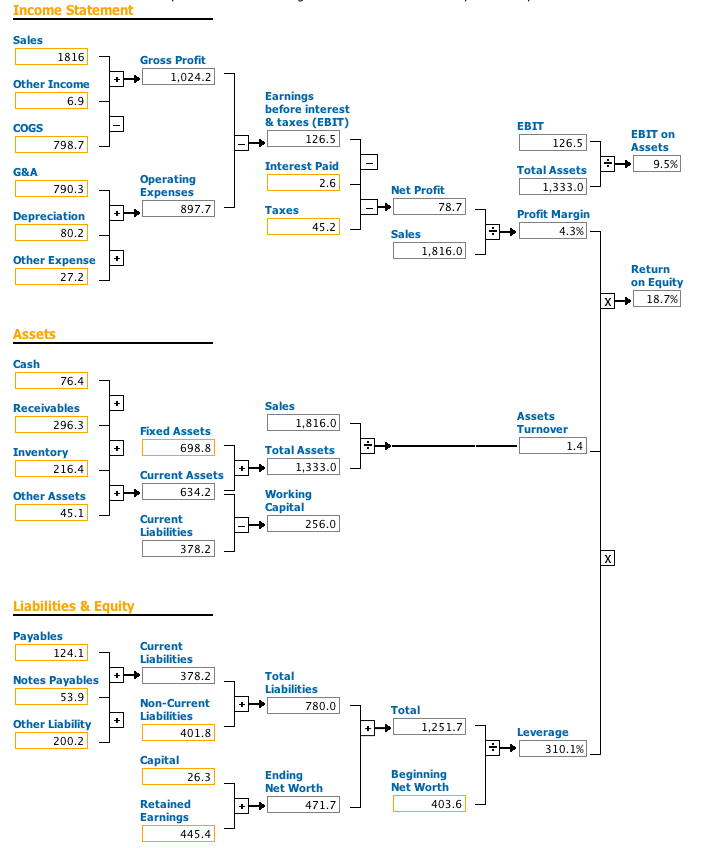
\includegraphics[height=8.6in]{dupont_chart.png}
	\caption{The DuPont Chart}
	\label{fig:dupont_chart}
\end{figure}

\section{Working Capital}
\begin{equation}
	\text{Working capital}
	= \text{Current assets} - \text{Short-term liabilities}
\end{equation}
Assure "working" of business without wasting short-term resources.

\subsection{Working Capital Management}
\begin{itemize}
	\item Cash Management
	\item Receivables Management
	\item Payables Management
	\item Inventory Management
\end{itemize}

\subsection{Cash Cycle}
\begin{eqnarray*}
	\text{Cash Cycle time} 
	&=&	\text{Inventory (Day)}\\
	&-& \text{Payables (Day)}\\ 
	&+& \text{Receivables (Day)}
\end{eqnarray*}

Use Capital Turnover (CTO) ratios to evaluate.

Cash invested in working capital has very low return

\section{Cash Flow}


\end{document}